%%%%%%%%%%%%%%%%%%%%%%%%%%%%%%%%%%%%%%%%%%%%%%%%%%%%%%%%%%%%%%%%%%%%%%%%%%%%%%%%
% Soutenance de projet - Fichier modèle pour présentations Beamer
%%%%%%%%%%%%%%%%%%%%%%%%%%%%%%%%%%%%%%%%%%%%%%%%%%%%%%%%%%%%%%%%%%%%%%%%%%%%%%%%
\documentclass{beamer}
\usepackage[utf8]{inputenc}
\usepackage[francais]{babel}
\usepackage[T1]{fontenc}
\usepackage{textcomp}
\usepackage{relsize}
\usepackage{amssymb}
\usepackage{framed}
\usepackage{makeidx}


%%% THÈME TORINO AVEC MINIFRAMES MODIFIÉES - NÉCESSITE FICHIERS SPÉCIAUX
\usetheme[pageofpages=sur,% String used between the current page and the
                         % total page count.
          alternativetitlepage=true,% Use the fancy title page.
          titlepagelogo=logo,% Logo for the first page.
          titleline=true,
          watermark=watermark,% Watermark used in every page.
          watermarkheight=100px,% Height of the watermark.
          watermarkheightmult=4,% The watermark image is 4 times bigger
                                % than watermarkheight.
          ]{Torino}
\useoutertheme[subsection=true]{miniframes2}
\usecolortheme{freewilly}
%%% FIN DU SECOND THÈME

% nouvelle commande pour un joli nom
\newcommand{\nom}[1]{\textsc{#1}}

% commande pour une zolie ligne
\newcommand{\ligne}[1][1pt]{
  \par\noindent
  \rule[.5ex]{\linewidth}{#1}\par}

% \0
\newcommand{\slz}{$\backslash0$}

\newcommand{\executeiffilenewer}[3]{%
 \ifnum\pdfstrcmp{\pdffilemoddate{#1}}%
 {\pdffilemoddate{#2}}>0%
 {\immediate\write18{#3}}\fi%
}

\newcommand{\includesvg}[2]{%
 %\executeiffilenewer{#1.svg}{#1.pdf}%
 %{inkscape -z -D --file=#1.svg --export-pdf=#1.pdf --export-width=1000}%
 %\input{#1.eps_tex}%
 \includegraphics[scale=#2]{#1.pdf}
}

\newcommand{\includedot}[2]{%
 \executeiffilenewer{#1.dot}{#1.pdf}%
 {dot -T pdf -o #1.pdf #1.dot}%
 %\input{#1.eps_tex}%
 \includegraphics[scale=#2]{#1.pdf}
}

\newcommand{\includepic}[2]{%
 \immediate\write18{pic2plot -Tsvg --bg-color none #1.pic > #1.svg && inkscape -z -D --file=#1.svg --export-pdf=#1.pdf --export-width=1000}%
 \includegraphics[scale=#2]{#1.pdf}
}

%%% TITRE DE PAGE
\title{Contextd Capture}
\subtitle{Capture d'activité système pour PIGA-SYSTRANS}
\author{Dimitri~Gressin \and Timothée~Ravier}
\institute{ENSI de Bourges}
\date{20 janvier 2011}

%%% POUR AVOIR UN PLAN QUI S'AFFICHE QUAND ON CHANGE DE SOUS-SECTION
\AtBeginSection[ ]
{
 \begin{frame}<beamer>
   \frametitle{Plan}
   \tableofcontents[currentsection]
  \end{frame}
}
\NoAutoSpaceBeforeFDP

\begin{document}

%%% LA PAGE DE TITRE, ON PEUT Y APPLIQUER DES OPTIONS COMME INSTITUTE CI-DESSOUS
{
	\framenumberoff
	\watermarkoff
	\institute{École Nationale Supérieure d'Ingénieurs de Bourges} % Vire le champ institut sur cette page
	\begin{frame}
	\titlepage
	\end{frame}
}

\section{Introduction}
\begin{frame}{Le context}
	\begin{enumerate}
		\item Contrôler les différents éléments accédés par les applications.
		\item Autoriser les actions en suivant une politique bien déterminer.
	\end{enumerate}
	~\\
	Jusqu'à présent : ~\\
	~\\
	\begin{enumerate}
		\item Plugin développé pour chaque application.
		\item Contextd.
	\end{enumerate}
\end{frame}

\begin{frame}{Schéma de fonctionnement initial}
	\begin{center}
			%\includesvg{attachements/contextd_dbus}{1}
			\includesvg{attachements/contextd_dbus}{.45}
	\end{center}
\end{frame}

\begin{frame}{Présentation du sujet}
	\begin{block}{But :}
		\textbf{Remplacer l'utilisation de plugin pour la plupart des applications.}
	\end{block}
	~\\
	Organisation du projet en quatre étapes : 
	\begin{itemize}
		\item[-] Intercepter les appels système
		\item[-] Récupérer des informations au niveau du noyau
		\item[-] Envoyer ces informations dans l'espace utilisateur à contextd
		\item[-] Retourner la réponse de contextd au noyau pour débloquer l'appel système
	\end{itemize}
\end{frame}

\section{Linux Security Modules}
\begin{frame}{Modules LSM}
	\begin{itemize}
		\item Ce sont des modules noyau
		\item Ils permettent de "hooker" les appels système
		\item Ils permettent d'interdire dynamiquement des appels système
	\end{itemize}
~\\	
\textbf{Les modules LSM répondent tout à fait à notre problématique}
\end{frame}

\begin{frame}
\frametitle{Schéma}
\begin{center}
	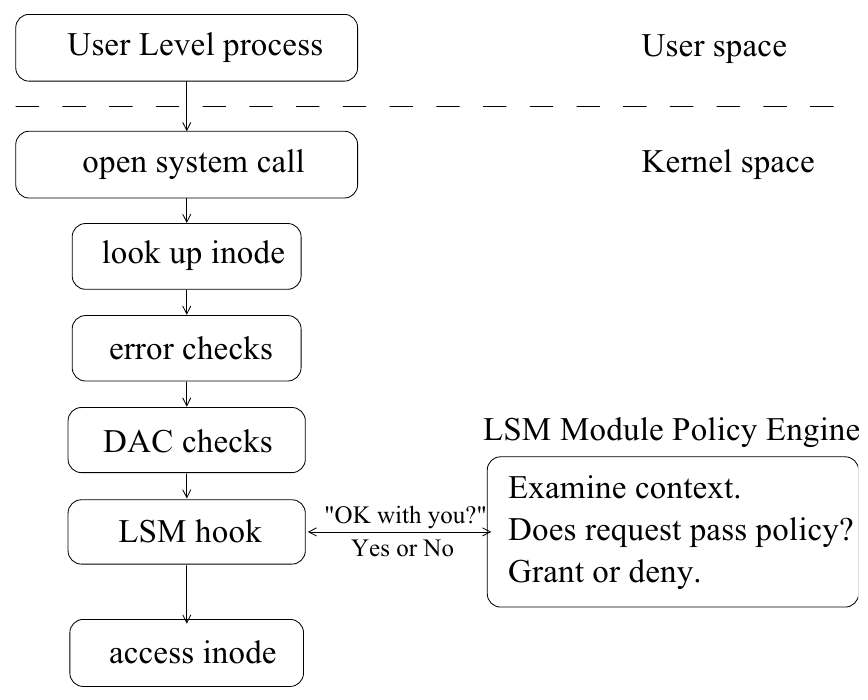
\includegraphics[scale=0.30]{attachements/lsm1.png}
\end{center}
\end{frame}


\section{Déroulement du projet}

\begin{frame}{Travail produit}
\begin{enumerate}
	\item Création du module LSM \\
	\begin{itemize}
		\item Création du module
		\item Création et implémentation des différents hooks \\
		\begin{itemize}
			\item file\_permission
			\item mkdir
			\item socket\_bind
			\item socket\_connect
			\item socket\_sendmsg
			\item socket\_recvmsg
		\end{itemize}
		\item Mise en place de verrou
	\end{itemize}	
	\item Ajout dans le mode de configuration standard du noyau
		\begin{itemize}
			\item Makefiles
			\item Kconfig
		\end{itemize}
\end{enumerate}
\end{frame}

\begin{frame}{Travail produit}
\begin{enumerate}
\setcounter{enumi}{2}
	\item Création de proc filesysstem \\
	\begin{itemize}
		\item Un dossier "contextd" (/proc/contextd/)
		\item Deux fichiers\
		\begin{itemize}
			\item /proc/contextd/status
			\item /proc/contextd/program
		\end{itemize}
	\end{itemize}
	\item Création de 3 appels systèmes \\
	\begin{itemize}
		\item auditsec\_register (int, char *);
		\item auditsec\_question (struct auditsec\_info *);
		\item auditsec\_answer (int);
	\end{itemize}
\end{enumerate}
\end{frame}

\begin{frame}{Diagramme de séquence}
	\begin{center}
		\includepic{attachements/sequence_diagram}{.6}
	\end{center}
\end{frame}

\begin{frame}{Travail produit}
\begin{enumerate}
\setcounter{enumi}{4}
	\item Modification de contextd \\
	\begin{itemize}
		\item Ajout d'une classe abstraire
		\begin{itemize}
			\item Gestion des clients ()
		\end{itemize}
		\item Modification de dbus-context
		\begin{itemize}
			\item Suppression de dbus\_id
			\item Indexation par pid
			\item Héritage avec abstractcontext
		\end{itemize}
		\item Ajout d'une classe kernel-context
		\begin{itemize}
			\item Hérite avec abstractcontext
			\item Thread d'écoute
		\end{itemize}
		\item Recharge des programmes surveillés dynamique (SIGUSR2)
	\end{itemize}
\end{enumerate}
\end{frame}

\begin{frame}{Diagramme de classes}
	\begin{center}
		\includedot{attachements/class}{.55}
	\end{center}
\end{frame}

\section{Résultats finaux}

\begin{frame}{Schéma global}
	\begin{center}
		\includesvg{attachements/fonctionnement_apres}{1}
	\end{center}
\end{frame}

\section{Remaques \& Amélioration}
\begin{frame}{Remarques \& Améliorations}
	\begin{itemize}
		\item Seuls les "hook" file\_permission et mkdir fonctionnent
		\item Acheminement des données pour les "hooks" réseau.
	\end{itemize}

	\begin{itemize}
		\item Gestion des "hooks" réseaux
		\item Cohabitation avec SELinux (en partie réalisée)
		\item Intégration à PIGA-OS
	\end{itemize}
\end{frame}

\section{Conclusion}
\begin{frame}
\frametitle{Conclusion}
\begin{itemize}
	\item[+] Objectifs globalement atteints
	\item[+] Partie système pleinement opérationnelle
\end{itemize} 
~\\
\begin{itemize}
	\item[-] L'intégration à SELinux
	\item[-] Partie réseau.
\end{itemize}
\end{frame}

\end{document}
